\pdfoutput=1

%\documentclass[preprint,10pt]{elsarticle}
\documentclass[10pt]{article}
%\documentclass[review]{siamart0216}

\usepackage{fullpage}
\usepackage{hyperref}
%\let\proof\relax
%\let\endproof\relax
\usepackage{amsmath,amssymb,amsfonts,mathrsfs}%,amsthm}
\usepackage[titletoc,toc,title]{appendix}

%\usepackage{lineno}
\usepackage{array} 
\usepackage[utf8]{inputenc}
\usepackage{listings}
\usepackage{mathtools}
\usepackage{pdfpages}
\usepackage[textsize=footnotesize,color=green]{todonotes}
\usepackage{bm}
%\usepackage{tikz}
\usepackage[normalem]{ulem}
\usepackage{hhline}

%% ====================================== alg package
\usepackage{algorithm}
\usepackage[noend]{algpseudocode}
\usepackage{algorithmicx}
\algblock{ParFor}{EndParFor}
% customising the new block
\algnewcommand\algorithmicparfor{\textbf{parfor}}
\algnewcommand\algorithmicpardo{\textbf{do}}
\algnewcommand\algorithmicendparfor{\textbf{end\ parfor}}
\algrenewtext{ParFor}[1]{\algorithmicparfor\ #1\ \algorithmicpardo}
\algrenewtext{EndParFor}{\algorithmicendparfor}
%% ====================================== end alg package

\usepackage{graphicx}
\usepackage{subfig}
\usepackage{color}

%% ====================================== graphics

\usepackage{pgfplots}
\usepackage{pgfplotstable}
\definecolor{markercolor}{RGB}{124.9, 255, 160.65}
\pgfplotsset{width=10cm,compat=1.9}
\pgfplotsset{
tick label style={font=\small},
label style={font=\small},
legend style={font=\small}
}

\usetikzlibrary{calc}
\usepackage{stmaryrd}


\renewcommand{\topfraction}{0.85}
\renewcommand{\textfraction}{0.1}
\renewcommand{\floatpagefraction}{0.75}

\newcommand{\vect}[1]{\ensuremath\boldsymbol{#1}}
\newcommand{\tensor}[1]{\underline{\bm{#1}}}
\newcommand{\del}{\triangle}
\newcommand{\curl}{\grad \times}
\renewcommand{\div}{\grad \cdot}
\newcommand{\td}[2]{\frac{{\rm d}#1}{{\rm d}{\rm #2}}}
\newcommand{\pd}[2]{\frac{\partial#1}{\partial#2}}
\newcommand{\pdd}[2]{\frac{\partial^2#1}{\partial#2^2}}

\newcommand{\bs}[1]{\boldsymbol{#1}}

\newcommand{\equaldef}{\stackrel{\mathrm{def}}{=}}

\newcommand{\tablab}[1]{\label{tab:#1}}
\newcommand{\tabref}[1]{Table~\ref{tab:#1}}

\newcommand{\theolab}[1]{\label{theo:#1}}
\newcommand{\theoref}[1]{\ref{theo:#1}}
\newcommand{\eqnlab}[1]{\label{eq:#1}}
\newcommand{\eqnref}[1]{\eqref{eq:#1}}
\newcommand{\seclab}[1]{\label{sec:#1}}
\newcommand{\secref}[1]{\ref{sec:#1}}
\newcommand{\lemlab}[1]{\label{lem:#1}}
\newcommand{\lemref}[1]{\ref{lem:#1}}

\newcommand{\mb}[1]{\mathbf{#1}}
\newcommand{\mbb}[1]{\mathbb{#1}}
\newcommand{\mc}[1]{\mathcal{#1}}
\newcommand{\nor}[1]{\left\| #1 \right\|}
\newcommand{\snor}[1]{\left| #1 \right|}
\newcommand{\LRp}[1]{\left( #1 \right)}
\newcommand{\LRs}[1]{\left[ #1 \right]}
\newcommand{\LRa}[1]{\left\langle #1 \right\rangle}
\newcommand{\LRb}[1]{\left| #1 \right|}
\newcommand{\LRc}[1]{\left\{ #1 \right\}}
\newcommand{\LRceil}[1]{\left\lceil #1 \right\rceil}

\newcommand{\Grad} {\ensuremath{\nabla}}
\newcommand{\Div} {\ensuremath{\nabla\cdot}}
\newcommand{\Nel} {\ensuremath{{N^\text{el}}}}
\newcommand{\jump}[1] {\ensuremath{\llbracket#1\rrbracket}}
\newcommand{\avg}[1] {\ensuremath{\LRc{\!\{#1\}\!}}}
\newcommand{\uh}{\widehat{u}}
\newcommand{\Bh}{\widehat{B}}
\newcommand{\fnh}{\widehat{f}_n}
\renewcommand{\L}{L^2\LRp{\Omega}}
\newcommand{\Lk}{L^2\LRp{D^k}}
\newcommand{\Dhat}{\widehat{D}}
\newcommand{\Lhat}{L^2\LRp{\Dhat}}
\newcommand{\pO}{\partial\Omega}
\newcommand{\Gh}{\Gamma_h}
\newcommand{\Gm}{\Gamma_{-}}
\newcommand{\Gp}{\Gamma_{+}}
\newcommand{\Go}{\Gamma_0}
\newcommand{\Oh}{\Omega_h}

%\newtheorem{theorem}{Theorem}[section]
%\newtheorem{lemma}[theorem]{Lemma}
%\newtheorem{proposition}[theorem]{Proposition}
%\newtheorem{corollary}[theorem]{Corollary}

%\newenvironment{definition}[1][Definition]{\begin{trivlist}
%\item[\hskip \labelsep {\bfseries #1}]}{\end{trivlist}}
%\newenvironment{example}[1][Example]{\begin{trivlist}
%\item[\hskip \labelsep {\bfseries #1}]}{\end{trivlist}}

\newcommand{\eval}[2][\right]{\relax
  \ifx#1\right\relax \left.\fi#2#1\rvert}

\def\etal{{\it et al.~}}


\def\arr#1#2#3#4{\left[
\begin{array}{cc}
#1 & #2\\
#3 & #4\\
\end{array}
\right]}
\def\vectwo#1#2{\left[
\begin{array}{c}
#1\\
#2\\
\end{array}
\right]}
\def\vecthree#1#2#3{\left[
\begin{array}{c}
#1\\
#2\\
#3\\
\end{array}
\right]}
\def\vectfour#1#2#3#4{\left[
\begin{array}{c}
#1\\
#2\\
#3\\
#4\\
\end{array}
\right]}

\newcommand{\G} {\Gamma}
\newcommand{\Gin} {\Gamma_{in}}
\newcommand{\Gout} {\Gamma_{out}}

\newcommand{\note}[1]{{\color{blue}#1}}
\newcommand{\remark}[1]{\textbf{\color{red}#1}}

\newcommand{\tri}{{\rm tri}}
\newcommand{\sqr}{{\rm quad}}

\newcommand{\refhex}{\widehat{\mathcal{H}}}
\newcommand{\reftet}{\widehat{\mathcal{T}}}
\newcommand{\refwedg}{\widehat{\mathcal{W}}}

\newcommand{\refpyr}{\widehat{\mathcal{P}}}
\newcommand{\refpyrf}{\widehat{\mathcal{P}}^f}
\newcommand{\refpyrfq}{\widehat{\mathcal{P}}^{\sqr}}
\newcommand{\refpyrft}{\widehat{\mathcal{P}}^{\tri}}


\newcommand{\hex}{{\mathcal{H}}}
\newcommand{\tet}{{\mathcal{T}}}
\newcommand{\wedg}{{\mathcal{W}}}

\newcommand{\pyr}{{\mathcal{P}}}
\newcommand{\pyrf}{{\mathcal{P}}^f}
\newcommand{\pyrfq}{{\mathcal{P}}^{\sqr}}
\newcommand{\pyrft}{{\mathcal{P}}^{\tri}}

\newcommand{\LinfDk}{L^{\infty}\LRp{D^k}}

\newcommand{\diag}[1]{{\rm diag}\LRp{#1}}

\newcommand{\half}{1/2}

\newcolumntype{C}[1]{>{\centering\let\newline\\\arraybackslash\hspace{0pt}}m{#1}}

%% d in integrand
\newcommand*\diff[1]{\mathop{}\!{\mathrm{d}#1}}

\makeatletter
\renewcommand\d[1]{\mspace{6mu}\mathrm{d}#1\@ifnextchar\d{\mspace{-3mu}}{}}
\makeatother

\newcommand{\squareface}{[-1,1]^2}

\date{}
\author{Jesse Chan, T. Warburton}
\title{On penalty flux parameters in first order DG formulations}

\begin{document}

\maketitle
%\tableofcontents

\begin{abstract}
Abstract goes here.  Mention assumptions: continuously varying material data, skew-symmetric formulations.  
\end{abstract}

\section{Introduction}

\note{Intro}

\section{DG numerical  fluxes}

We consider a first order system of hyperbolic equations
\[
\bm{A}_0\pd{\bm{U}}{t} + \sum_{i=1}^d \pd{\bm{F}_i(\bm{U})}{\bm{x}_i} = 0,
\]
which may alternatively be written as
\[
\bm{A}_0\pd{\bm{U}}{t} + \sum_{i=1}^d \pd{\LRp{\bm{A}_{i}U}}{\bm{x}_i}, \qquad \bm{A}_{i} = \pd{\bm{F}_i(\bm{U})}{\bm{U}}
\]
where $\bm{A}_{i}$ are symmetric matrices.  The semi-discrete DG formulation for such systems may be written as 
\[
\sum_{D^k \in \Oh} \LRp{\bm{A}_0\pd{\bm{U}}{t},\bm{V} }_{\Lk} = \sum_{D^k \in \Oh}\LRp{ \LRp{\bm{F}_i(\bm{U}), \bm{V}_{,i}}_{\Lk} - \LRa{\bm{F}_n^*(\bm{U})\bm{n}_i,\bm{V}}_{\partial D^k}}
\]
where $\bm{n}$ is the outward normal on a face $f$ of $D^k$, and $\bm{F^*}_n$ is a numerical flux depending defined on shared faces between two elements.  

\note{Define $\Oh, \Gh$, derive global formulation.}  

%For convergence, $\bm{F^*}_n = \bm{F^*}_n(\bm{U})$ must be consistent such that, for exact solutions $\bm{U}$, 
%\[
%\bm{F^*}_n = \bm{F}(\bm{U})\cdot \bm{n}.
%\]

Let $f$ be a shared face between two elements $D^{k,+}$ and $D^{k,-}$, and let $\bm{F}^+, \bm{F}^-$ be evaluations of $\bm{F}(\bm{U})$ restricted to $D^{k,+}$ and $D^{k,-}$, respectively.  The average and jump of a vector valued function over $f$ are then defined as
\[
\avg{\bm{F}} = \frac{\bm{F}^+ + \bm{F}^-}{2}, \qquad \jump{\bm{F}} = \bm{F}^+ - \bm{F}^-.
\]
Typical numerical fluxes are defined as the sum of the average of $\bm{F}^+$ and $\bm{F}^-$ and a penalization term $\bm{G(\bm{U}^+,\bm{U}^-)}$
\begin{equation}
\bm{F^*}_n = \avg{\bm{F}(\bm{U})}\cdot \bm{n} - \bm{G(\bm{U}^+,\bm{U}^-)}.
\label{eq:flux}
\end{equation}

The upwind numerical flux is a well-known flux of the form (\ref{eq:flux}).  For an outward normal vector $\bm{n}$, let ${\bm{A}}_n = \sum_{i=1}^d {\bm{A}_i\bm{n}_i}$.  By \note{add citation}, ${\bm{A}}_n$ contains real eigenvalues, and admits an eigenvalue decomposition
\[
\bm{A}_n = \bm{V}{\bm{\Lambda}}\bm{V}^T, \qquad \bm{\Lambda} = 
\left(\begin{array}{ccc}
\lambda_1 & & \\
& \ddots & \\
& & \lambda_d
\end{array}\right).
\]
For problems with continuous coefficients, the upwind numerical flux over a face $f \in \Gh$ can be defined  as
\[
\bm{F^*}_n = \bm{A}_n^+\bm{U}^- + \bm{A_n}^- \bm{U}^+,
\]
where the matrices $\bm{A_n}^+,\bm{A_n}^-$ are constructed from the positive and negative eigenvalues 
\begin{align*}
\bm{A}_n^+ &= \frac{1}{2}\bm{V} \LRp{\bm{\Lambda} + \LRb{\bm{\Lambda}}} \bm{V}^T\\
\bm{A}_n^- &= \frac{1}{2}\bm{V} \LRp{\bm{\Lambda} - \LRb{\bm{\Lambda}}} \bm{V}^T,
\end{align*}
and $\LRb{\bm{\Lambda}}$ is the diagonal matrix whose entries consist of the absolute values of the eigenvalues $\LRb{\lambda_i}$.  This can be rewritten as the sum of the central flux and a penalization
\[
\bm{F^*}_n = \avg{\bm{A}_n\bm{U}} - \bm{V}\LRb{\bm{\Lambda}}\bm{V}^T \jump{\bm{U}}.  
\]
For problems with discontinuous coefficients, this may be generalized by solving a Riemann problem to yield
\[
\bm{F^*}_n = \avg{\bm{A}_n\bm{U}} - \jump{{\bm{V}\LRb{\bm{\Lambda}}\bm{V}^T\bm{U}}}.  
\]
An alternative to upwind fluxes are penalty fluxes, which penalize appropriately defined jumps of the solution.  One such penalty flux is 
\[
\bm{F^*}_n = \avg{\bm{A}_n\bm{U}} - \tau \bm{A}_n^T \jump{\bm{A}_n\bm{U}}.  
\]
where $\tau$ is proportional to $\lambda_{\max}^{-1}$.  This choice of $\tau$ ensures that the penalty term is of the same order of magnitude as the upwind penalization, and that the CFL restriction for both methods is identical.  

\note{Skew-symmetric discretization for constant coefficient problems \cite{kopriva2014energy}.  Extendable to Maxwells \cite{warburton2013low} and elasticity \cite{wilcox2010high,ye2016discontinuous}.}

\subsection{Conforming and non-conforming spaces}


Let $V$ denote the piecewise polynomial approximation space 
\[
V = \LRc{ \bm{U} \in\LRp{ L^2(\Oh)}^d : \left.\bm{U}\right|_{D^k} \in \LRp{P^N(D^k)}^d}.  
\]
We define a decomposition of $V$ into a conforming part $V^C$ and a non-conforming part $V^{NC}$ based on the penalization term $\bm{G}(\bm{U}^+,\bm{U}^-)$.  The conforming part is defined as the null space of $\bm{G}(\bm{U}^+,\bm{U}^-)$
\begin{equation}
V^{C} = \LRc{ \bm{U}(\bm{x}) \in V: \quad  \bm{G}(\bm{U}^+,\bm{U}^-) = 0, \quad \forall f \in \Gh},
\label{eq:conf}
\end{equation}
while the non-conforming approximation space $V^{NC}$ is defined as $L^2$ orthogonal complement of $V^{C}$ in $V$
\[
V^{NC} = \LRc{ \bm{U}(\bm{x}) \in V: \LRp{\bm{u},\bm{v}}_{L^2(\Oh)} = 0, \quad \forall \bm{v}\in V^C}.
\]
\note{For problems where $\bm{A}_i$ are spatially continuous, $\bm{V}\LRb{\bm{\Lambda}}\bm{V}^T \jump{\bm{U}} = 0$ if and only if $\bm{A}_n^T \bm{A}_n\jump{\bm{U}} = 0$.  Both conditions enforce that 
\[
\bm{v}_i^T \jump{\bm{U}} = 0, \qquad \lambda_i \neq 0.
\]
}
As a result, the conforming and non-conforming spaces induced by upwind and penalty fluxes are identical.  

For problems with discontinuous material data, it is less straightforward to show equivalence between the conforming spaces $V^C$ resulting from upwind and penalty fluxes.  However, for many practical wave propagation settings, spatially varying coefficients are incorporated into the matrix $\bm{A_0}$, resulting in constant $\bm{A}_i$.  For both smoothly varying and discontinuous $\bm{A}_0$, it is possible to formulate energy stable DG methods with penalty fluxes \cite{mercerat2015nodal, chan2016weight1}.  Additionally, DG methods using penalty fluxes are observed to perform similarly to DG methods with upwind fluxes for  wave propagation problems with discontinuous coefficients \cite{warburton2013low, chan2016weight1, ye2016discontinuous}.  

\subsection{Scalar advection and acoustic wave propagation}
\label{sec:confexamples}
We illustrate the conforming spaces induced by penalty fluxes using the scalar advection equation and acoustic wave equation as concrete examples.  The scalar advection equation is given as
\[
\pd{u}{t} + \div\LRp{\bm{\beta}u} = 0.
\]
where $\bm{\beta}$ is the direction of advection.  For continuous advection vectors such that $\bm{\beta}(\bm{x}) \neq 0$, the penalty flux is equivalent to a parametrized upwind flux \cite{hesthaven2007nodal}
\[
\bm{F}^*_n = \avg{\bm{\beta}_n u} - \tau\LRb{\bm{\beta}_n}\jump{u}.
\]
The conforming space $V^C$ induced by this flux is then
\[
V^C = \LRc{ u \in L^2\LRp{\Oh} : \quad \left.u\right|_{D^k} \in P^N(D^k), \quad \LRb{\bm{\beta}_n}\jump{u} = 0}.
\]
In one dimension, this simply implies that $u$ is $C^0$ continuous across element boundaries.  In higher dimensions, this implies that $u$ is continuous along streamlines or directions $\bm{d}(\bm{x})$ where $\bm{\beta}\cdot \bm{d} \neq 0$.  

Next, we consider the acoustic wave equation in pressure-velocity form
\begin{align*}
\frac{1}{c^2}\pd{p}{t} &= \Div \bm{u}\\
\pd{\bm{u}}{t} &= \Grad p,
\end{align*}
where $c^2(\bm{x})$ is the wavespeed.  Let $\bm{U}$ denote the group variable $\bm{U} = (p,u,v)$, where $u$ and $v$ are the $x$ and $y$ components of velocity.  Then, in two dimensions, the isotropic wave equation is given as
\[
\pd{\bm{U}}{t} + \pd{\bm{A}_x\bm{U}}{x} + \pd{\bm{A}_y\bm{U}}{y} = 0, \qquad \bm{A}_x = 
\left(\begin{array}{ccc}
0 & 1 & 0\\
1 & 0 & 0\\
0 & 0 & 0
\end{array}
\right), \qquad 
\bm{A}_y = 
\left(\begin{array}{ccc}
0 & 0 & 1\\
0 & 0 & 0\\
1 & 0 & 0
\end{array}
\right).
\]
The normal flux matrix $\bm{A}_n$ is then
\[
\bm{A}_n = 
\left(\begin{array}{ccc}
0 & \bm{n}_x & \bm{n}_y\\
\bm{n}_x & 0 & 0\\
\bm{n}_y & 0 & 0
\end{array}
\right)
\]
implying that the penalty fluxes (with $\bm{W} = \tau\bm{I}$) are 
\[
\avg{\bm{A}_n \bm{U}} - \tau\bm{A}_n^T \jump{\bm{A}_n\bm{U}} = \left(\begin{array}{c}
\avg{\bm{u}_n}\\
\avg{p }\bm{n}_x\\
\avg{p }\bm{n}_y
\end{array}
\right) - 
\tau\left(\begin{array}{c}
\jump{p}\\
\jump{\bm{u_n}}\bm{n}_x\\
\jump{\bm{u_n}}\bm{n}_y
\end{array}
\right)
\]
For $\tau = 1$, these fluxes coincide with the upwind fluxes for continuously varying media.  In this case, the conforming subspace $V^{C}$ induced by the penalty flux consists of a scalar (pressure) component $V^C_p$ and a vector (velocity) component $V^C_{\bm{u}}$.  The pressure component $p$ satisfies $\jump{p} = 0$ over all faces $f\in \Gh$.  For polynomial approximation spaces, this implies that $p$ is continuous across faces, edges, and vertices, and $V^C_p$ is the standard $C^0$ continuous piecewise polynomial finite element space.  For the velocity component of $V^C$, the penalty fluxes enforce normal continuity, such that $\jump{\bm{u}}\cdot \bm{n} = 0$ over all faces $f \in \Gh$.  Since each component of $\bm{u}$ is approximated from $P^N(D^k)$, this implies that $V^C_{\bm{u}}$ is the $H({\rm div})$-conforming Brezzi-Douglas-Marini finite element space \cite{brezzi1985two,boffi2013mixed}.\footnote{It is possible to recover $V^C_{\bm{u}}$ as the Raviart-Thomas finite element space by approximating each component of $\bm{u}$ from a smaller polynomial space \cite{kirby2004algorithm}.}  

Penalty fluxes can also be interpreted as Lax-Friedrichs fluxes applied to scalar and vector variables separately.  In contrast, for a component-wise Lax-Friedrichs flux 
\[
\avg{\bm{A}_n \bm{U}} - \tau\bm{A}_n^T \jump{\bm{A}_n\bm{U}} = \left(\begin{array}{c}
\avg{\bm{u}_n}\\
\avg{p }\bm{n}_x\\
\avg{p }\bm{n}_y
\end{array}
\right) - 
\tau\left(\begin{array}{c}
\jump{p}\\
\jump{\bm{u}_x}\\
\jump{\bm{u}_y}
\end{array}
\right),
\]
the conforming space $V^C_{\bm{u}}$ becomes the space of vector piecewise polynomial functions which are $C^0$ continuous in both components, resulting in overly-constrained continuity conditions for $\bm{u}$.  


\section{Dependence of spectra on the penalty parameter}

\note{Define spaces and show that $\bm{S}$ is symmetric definite based on DG discretization.}  

We adapt the proof presented in \cite{Warburton20063205} to show that the spectra of $\bm{K}$ splits into two sets as $\tau\rightarrow \infty$, the first of which approaches the eigenvalues of $\bm{A}$, and the second of which moves left of the imaginary axis at a rate of $O(\tau)$.  

\note{finish}
This induces a block decomposition
\[
\bm{K} = \left(\begin{array}{cc}
\bm{A} & \bm{B}\\
-\bm{B}^T & \bm{C} + \tau \bm{S}
\end{array}\right).
\]
We first consider the spectra of $\bm{C} + \tau\bm{S}$.  By the construction of the DG formulation $\bm{C}$ is skew-symmetric, while $\bm{S}$ is symmetric and negative-definite.  Let $\lambda, \bm{u}$ be an eigenpair of $\bm{C} + \tau{\bm{S}}$ corresponding to the largest $N^D$ eigenvalues. Let $\lambda = \alpha + i\beta$ and $\bm{u} = \bm{v} + i\bm{w}$, where $\alpha,\beta$ and $\bm{v},\bm{w}$ are the real and imaginary parts of $\lambda$ and $\bm{u}$, respectively.  Then, expanding and grouping terms in
\[
(\bm{C}+\tau\bm{S})(\bm{v} + i\bm{w}) = (\alpha + i\beta) (\bm{v} + i\bm{w})
\]
we have that
\begin{align*}
(\bm{C}+\tau\bm{S})\bm{v} &= \alpha\bm{v}-\beta\bm{w}\\
(\bm{C}+\tau\bm{S})\bm{w} &= \beta\bm{v}+\alpha\bm{w}.
\end{align*}
Assuming that $\nor{\bm{u}}^2 = \nor{\bm{v}}^2 + \nor{\bm{w}}^2 = 1$, multiplying both sides by $\bm{v}^T,\bm{w}^T$ and straightforward manipulations %yield
%\begin{align*}
%\bm{v}^T\bm{A}\bm{v} &= \alpha\nor{\bm{v}}^2-\beta\bm{v}^T\bm{w}\\
%\bm{w}^T\bm{A}\bm{w} &= \beta\bm{w}^T{\bm{v}}+\alpha\nor{\bm{w}}^2.  
%\end{align*}
%\begin{align*}
%\bm{v}^T\bm{A}\bm{v} + \bm{w}^T\bm{A}\bm{w} &= \alpha\\
%\bm{v}^T\bm{A}\bm{w} - \bm{w}^T\bm{A}\bm{w} &= \beta.
%\end{align*}
using the skew-symmetry of $\bm{C}$ and symmetry of $\bm{S}$ yields
\begin{align*}
\bm{v}^T\bm{C}\bm{w} - \bm{w}^T\bm{C}\bm{w} &= \beta\\
\tau\LRp{\bm{v}^T\bm{S}\bm{v} + \bm{w}^T\bm{S}\bm{w}} &= \alpha.
\end{align*}
Since $\bm{v}^T\bm{C}\bm{w} - \bm{w}^T\bm{C}\bm{w}= 2\bm{w}^T\bm{C}\bm{v} = \beta$ is independent of $\tau$ and $\bm{v},\bm{w}$ are normalized, $\beta$ remains bounded as $\tau\rightarrow \infty$.  Similarly, since $\bm{S}$ is symmetric, negative-definite, and independent of $\tau$, the quantity
\[
\LRb{\bm{v}^T\bm{S}\bm{v} + \bm{w}^T\bm{S}\bm{w}} = \LRb{\frac{\alpha}{\tau}}
\]
is bounded independently of $\tau$, and we conclude that $\LRb{\alpha} = O(\tau)$.  Thus, as $\tau$ increases, the eigenvalues of $\bm{C} + \tau\bm{S}$ are shifted further and further left of the imaginary axis.  

We may now show how the spectra of $\bm{K}$ behaves as $\tau \rightarrow \infty$.  Following \cite{Warburton20063205}, let $\bm{U}$ and $\bm{Q}$ be unitary matrices whose columns contain the eigenvectors of $\bm{A}$ and $\bm{C} + \tau \bm{S}$, respectively.  Then, applying a block diagonal similarity transform yields
\[
\left(\begin{array}{cc}
\bm{U}^* & \\
& \bm{Q}^*
\end{array}\right)
\left(\begin{array}{cc}
\bm{A} & \bm{B}\\
-\bm{B}^T & \bm{C} + \tau \bm{S}
\end{array}\right)
\left(\begin{array}{cc}
\bm{U} & \\
& \bm{Q}
\end{array}\right)
 = \left(\begin{array}{cc}
\bm{\Lambda}_C & \bm{U}^T\bm{B}\bm{Q}\\
-\bm{Q}^T\bm{B}^T\bm{U} & \bm{\Lambda}_D
\end{array}\right),
\]
where $\bm{\Lambda}_C,\bm{\Lambda}_D$ are diagonal matrices whose entries consist of eigenvalues of $\bm{A},\bm{C} + \tau\bm{S}$, respectively.  Since $\bm{B}$ is independent of $\tau$, $\nor{\bm{U}^T\bm{B}\bm{Q}}$ can be bounded independently of $\tau$, assuming that $\bm{U}$ and $\bm{Q}$ are normalized.  Gerschgorin's theorem applied to $\bm{\Lambda}_C,\bm{\Lambda}_D$ then implies that the eigenvalues of $\bm{K}$ are contained in two sets of discs with radii independent of $\tau$.  The first set of discs are centered around $\lambda^C_i$ for $i = 1,\ldots,N^C$, while the second set of discs are centered around $\lambda^D_i$ for $i = 1,\ldots,N^D$, where ${\rm Re}(\lambda^D_i) = O(\tau)$. 

Consider now the $N^C$ eigenvalues with the smallest magnitude.  By the Gerschgorin argument, these must remain bounded as $\tau \rightarrow \infty$.  Let $\bm{W} = (\bm{W}_C,\bm{W}_D)$ and $\bm{\Lambda}_C$ be the matrix of eigenvectors and eigenvalues corresponding to these $N^C$ smallest eigenvalues, such that
\[
\left(\begin{array}{cc}
\bm{A} & \bm{B}\\
-\bm{B}^T & \bm{C} + \tau \bm{S}
\end{array}\right)
\left(\begin{array}{c}
\bm{W}_C
\\
\bm{W}_D
\end{array}\right) = 
\left(\begin{array}{c}
\bm{A}\bm{W}_C + \bm{B}\bm{W}_D\\
-\bm{B}^T\bm{W}_C + \bm{C}\bm{W}_D + \tau \bm{S}\bm{W}_D
\end{array}\right)
= 
\bm{\Lambda}_C
\left(\begin{array}{c}
\bm{W}_C
\\
\bm{W}_D
\end{array}\right) 
\]
This implies 
\[
\tau \nor{\bm{S}\bm{W}_D} = \nor{\bm{\Lambda}_C \bm{W}_D + \bm{B}^T\bm{W}_C  - \bm{C}\bm{W}_D}.
\]
Since $\Lambda_C$ remains bounded as $\tau\rightarrow \infty$, the right hand side is bounded independently of $\tau$ under normalization of $\bm{W}_C,\bm{W}_D$, implying that the non-conforming component $\bm{W}^D$ satisfies
\[
C\nor{\bm{W}_D} \leq \nor{\bm{S}\bm{W}_D} = O(1/\tau).
\]
As a consequence, $\bm{W}_D \rightarrow 0$ as $\tau\rightarrow \infty$, and the smallest $N^C$ eigenvalues of $\bm{K}$ converge to the purely imaginary eigenvalues of $\bm{A}$ at a rate of $O(1/\tau)$.  These correspond to a discretization using the conforming approximation space (\ref{eq:conf}).

\section{Numerical experiments}

The above analysis illustrates the behavior of the spectra of the DG discretization for the asymptotic cases when $\tau = 0$ or $\tau \rightarrow \infty$.  However, it is less clear how the spectra of $\bm{K}$ behaves for $\tau = O(1)$.  We rely instead on numerical experiments in one and two space dimensions to illustrate behaviors for the advection and acoustic wave equations.  

\subsection{1D experiments}

We consider first the scalar advection equation in 1D with periodic boundary conditions.  For $\tau = 0$, the eigenvalues of the DG discretization matrix are purely imaginary.  Paths taken by eigenvalues as $\tau$ increases are determined by sampling spectra over a sufficiently fine set of $\tau$ and using a particle tracking method \cite{simpletracker}.  Figure~\ref{fig:track1D} shows the paths taken by these eigenvalues as $\tau$ increases from zero to $\tau = 4$.  As predicted, a subset of \emph{divergent} eigenvalues move further left of the imaginary axis as $\tau$ increases.  The corresponding eigenmodes are shown in Figure~\ref{fig:trackmodes1D}, with inter-element jumps of these eigenfunctions increasing as $\tau$ increases.  

\begin{figure}
\centering
\subfloat[Paths of eigenvalues as $\tau$ increases]{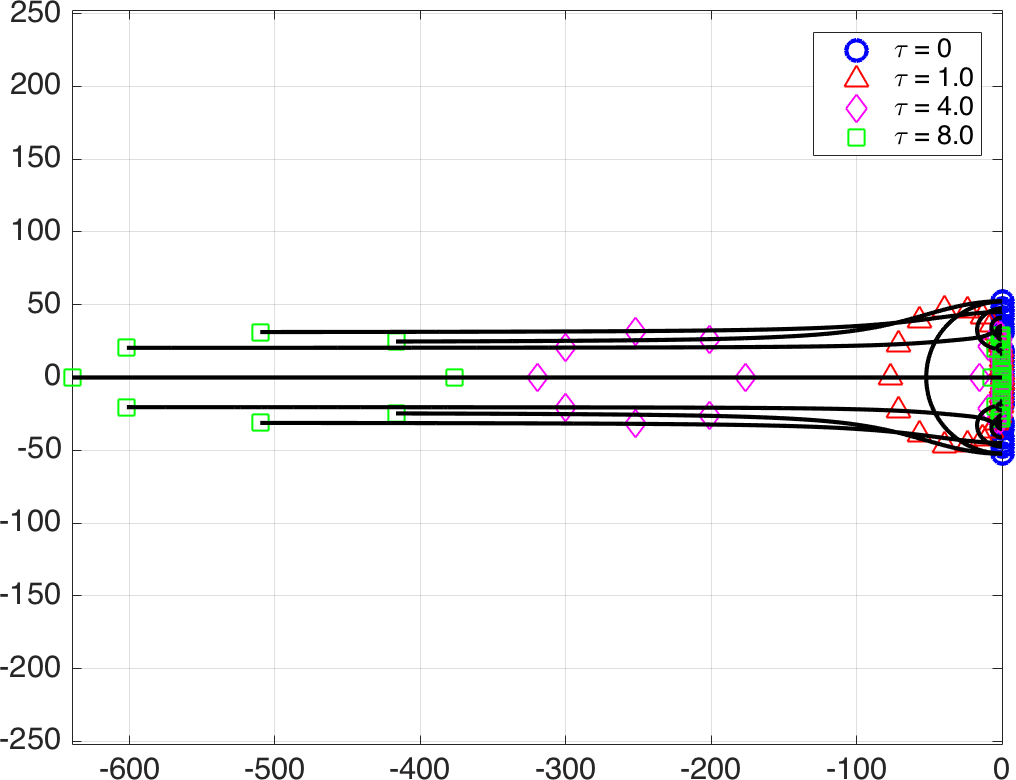
\includegraphics[width=.46\textwidth]{figs/trackedEigs.png}}
\hspace{1em}
\subfloat[Zoom of eigenvalues near imaginary axis]{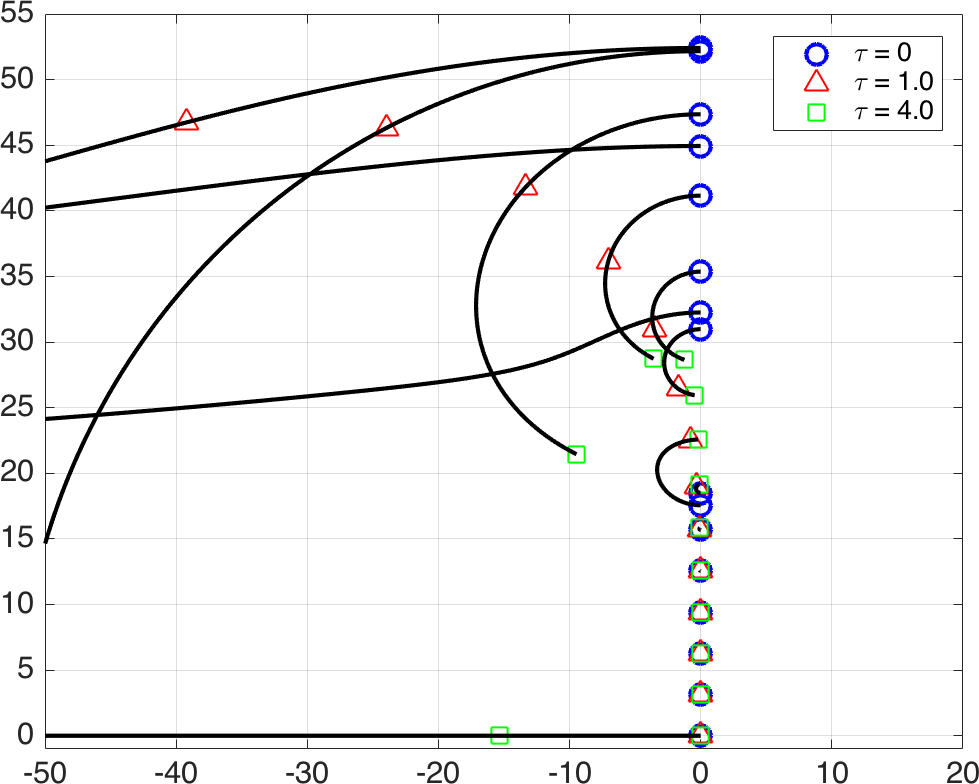
\includegraphics[width=.44\textwidth]{figs/trackedEigsZoom.png}}
\caption{Eigenvalue paths for DG advection with $\tau \in [0,4]$ on a mesh of 8 elements of degree $N=3$.  Eigenvalues are overlaid on these paths for $\tau = 0$, $\tau = 1$, and $\tau = 4$.  The zoomed in view near the imaginary axis shows the return of spurious modes to the imaginary axis for $\tau$ sufficiently large. }
\label{fig:track1D}
\end{figure}

\begin{figure}
\centering
\subfloat{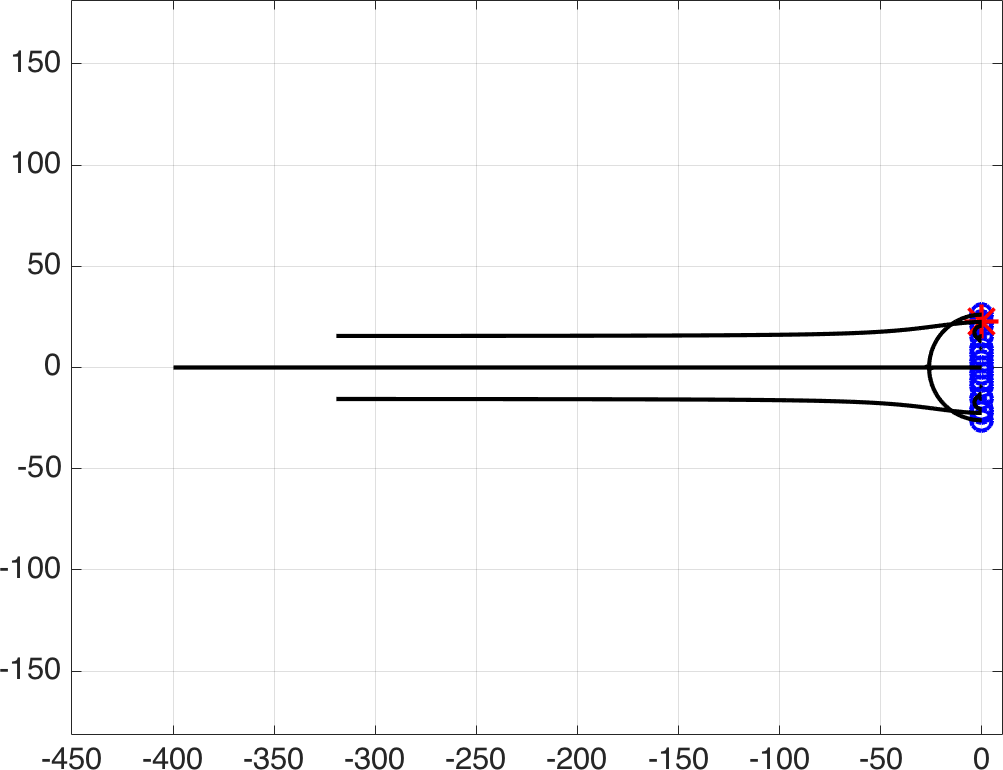
\includegraphics[width=.32\textwidth]{figs/tauEigsDiverge1.png}}
\hspace{.5em}
\subfloat{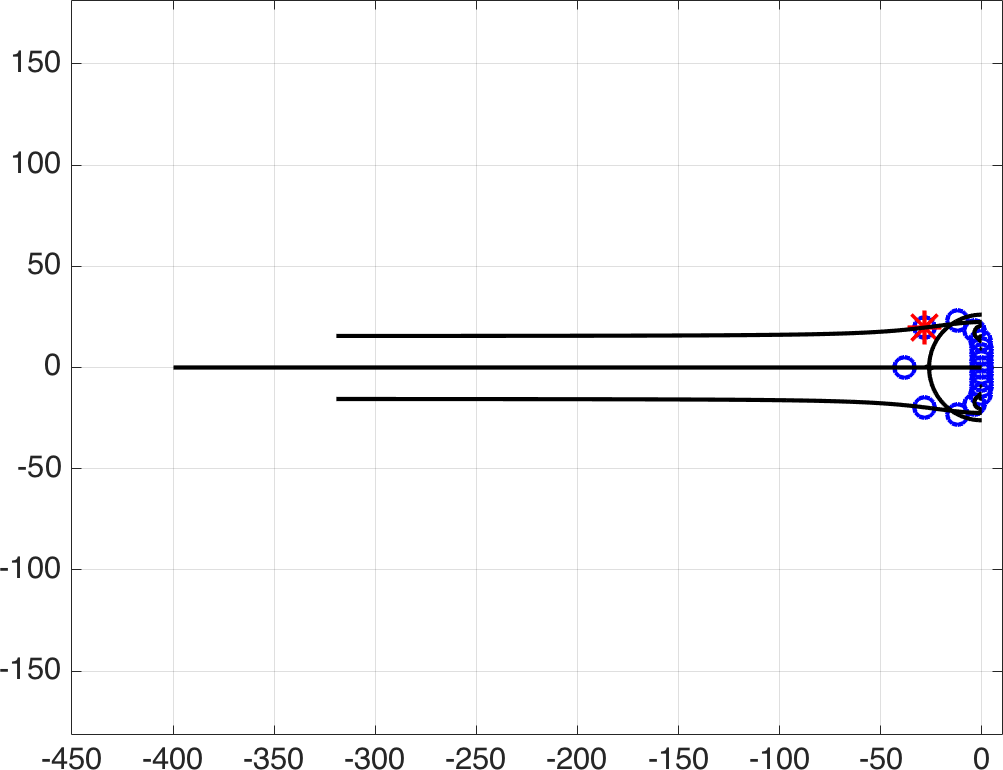
\includegraphics[width=.32\textwidth]{figs/tauEigsDiverge2.png}}
\hspace{.5em}
\subfloat{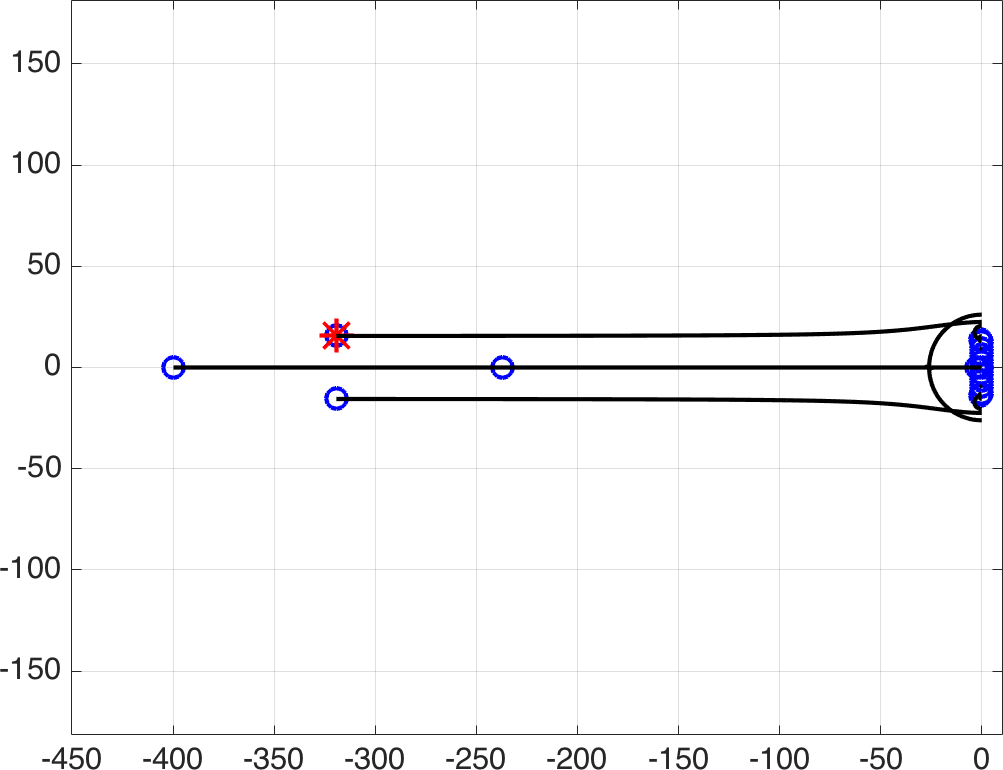
\includegraphics[width=.32\textwidth]{figs/tauEigsDiverge3.png}}\\
\subfloat[$\tau = 0$]{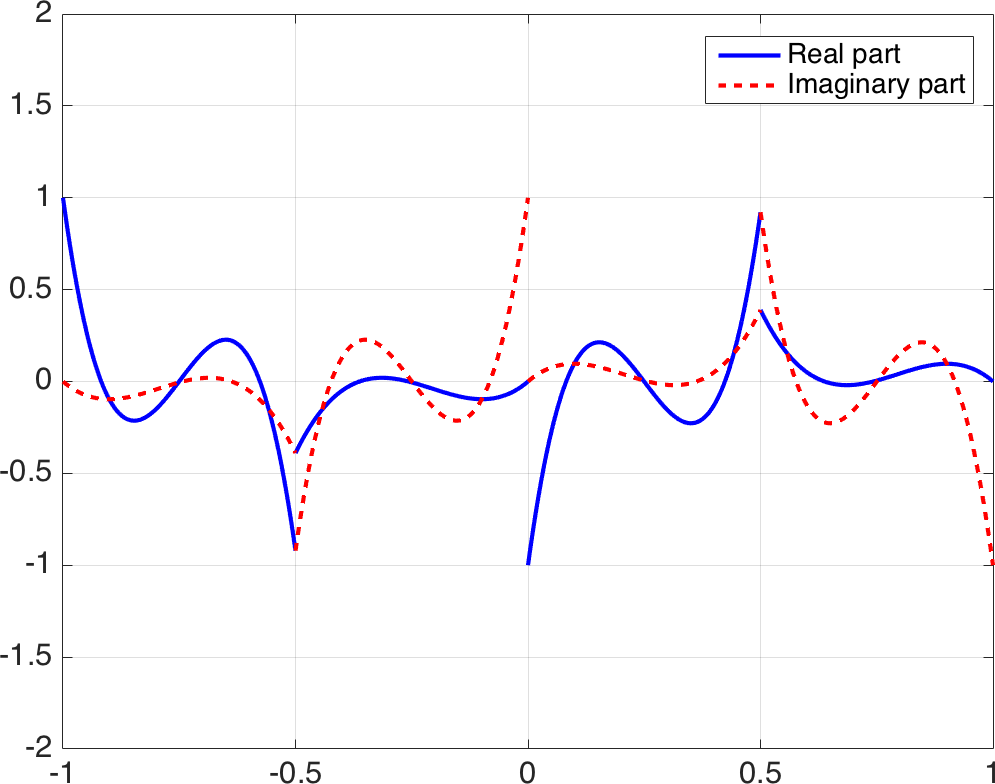
\includegraphics[width=.32\textwidth]{figs/tauModesDiverge1.png}}
\hspace{.5em}
\subfloat[$\tau = 1$]{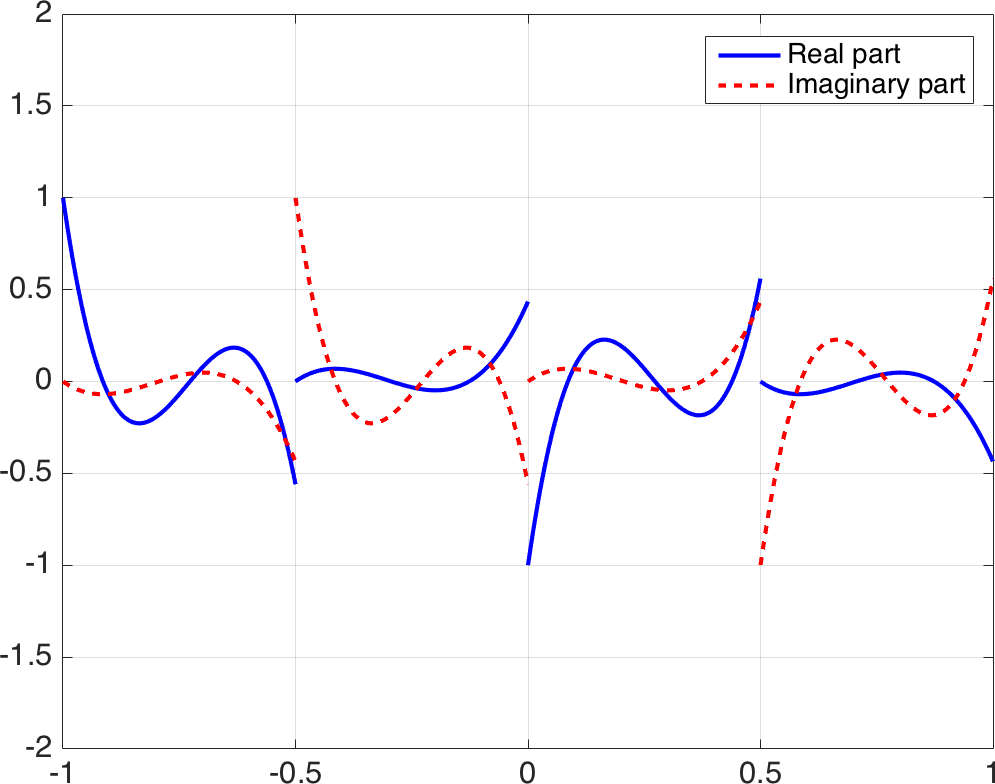
\includegraphics[width=.32\textwidth]{figs/tauModesDiverge2.png}}
\hspace{.5em}
\subfloat[$\tau = 10$]{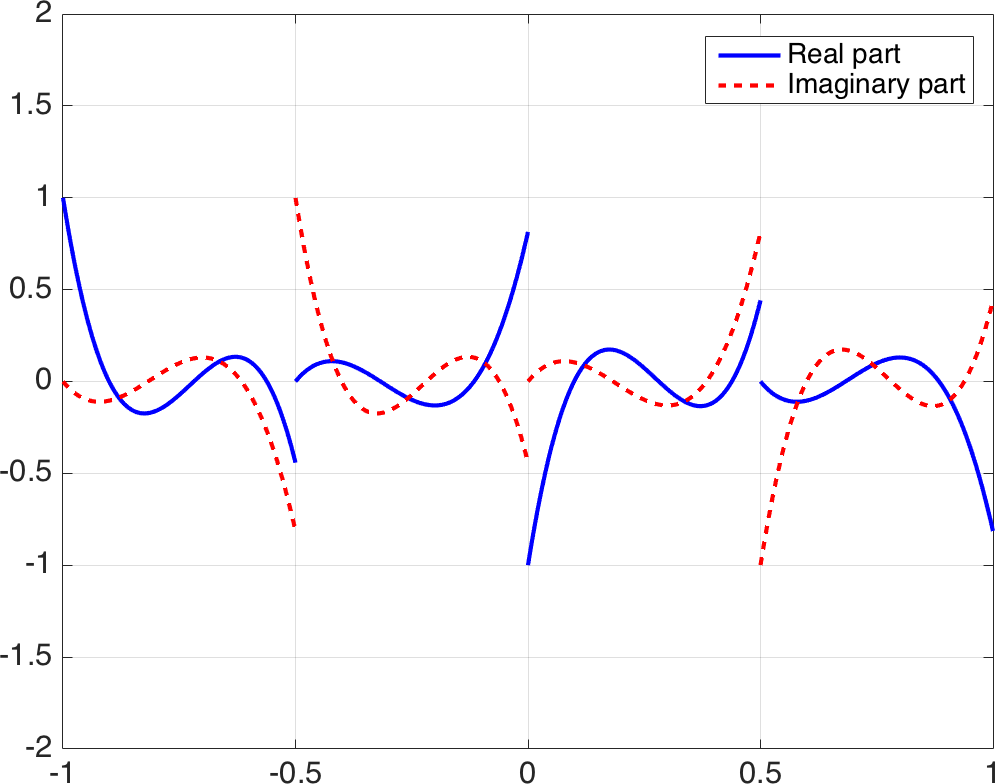
\includegraphics[width=.32\textwidth]{figs/tauModesDiverge3.png}}
\caption{Behavior of divergent eigenvalues for advection as $\tau$ increases.  The order of approximation is $N=3$ on a mesh of 4 elements.} %The displayed eigenfunctions correspond to the highlighted eigenvalue.  }
\label{fig:trackmodes1D}
\end{figure}

However, for sufficiently large $\tau$, a subset of eigenvalues return to the imaginary axis.  Figure~\ref{fig:spurious} illustrates that, as $\tau$ increases, the magnitude of the inter-element jumps present in these modes decreases, and the mode approaches a $C^0$ continuous function.  These eigenvalues which move right to return to the imaginary axis correspond to a second set of \emph{spurious} modes.  These spurious modes, corresponding to under-resolved modes of the exact underlying operator, consist of higher frequency components with sharp peaks and have previously been observed in high order $C^0$ finite element methods \cite{ainsworth2014dispersive,hughes2014finite}.  

\begin{figure}
\centering
\subfloat{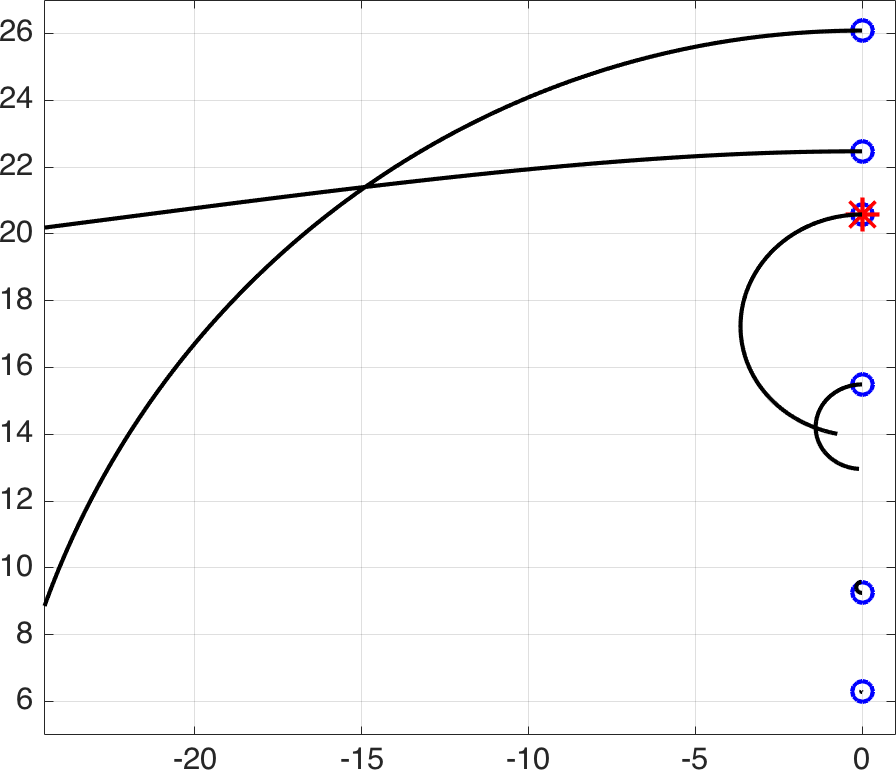
\includegraphics[width=.32\textwidth]{figs/tauEigs1.png}}
\hspace{.5em}
\subfloat{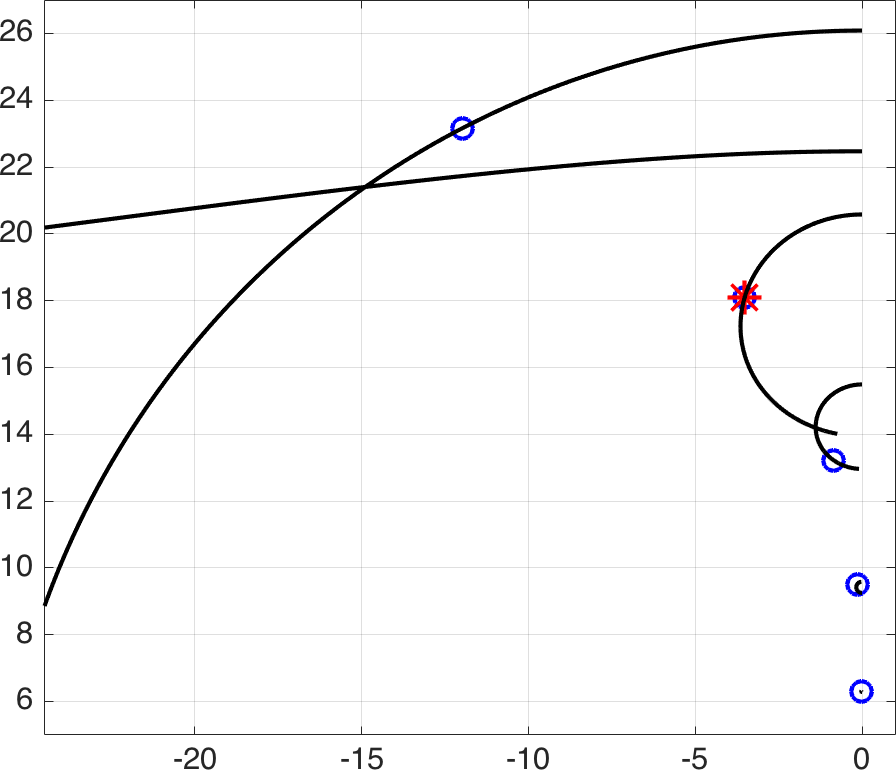
\includegraphics[width=.32\textwidth]{figs/tauEigs2.png}}
\hspace{.5em}
\subfloat{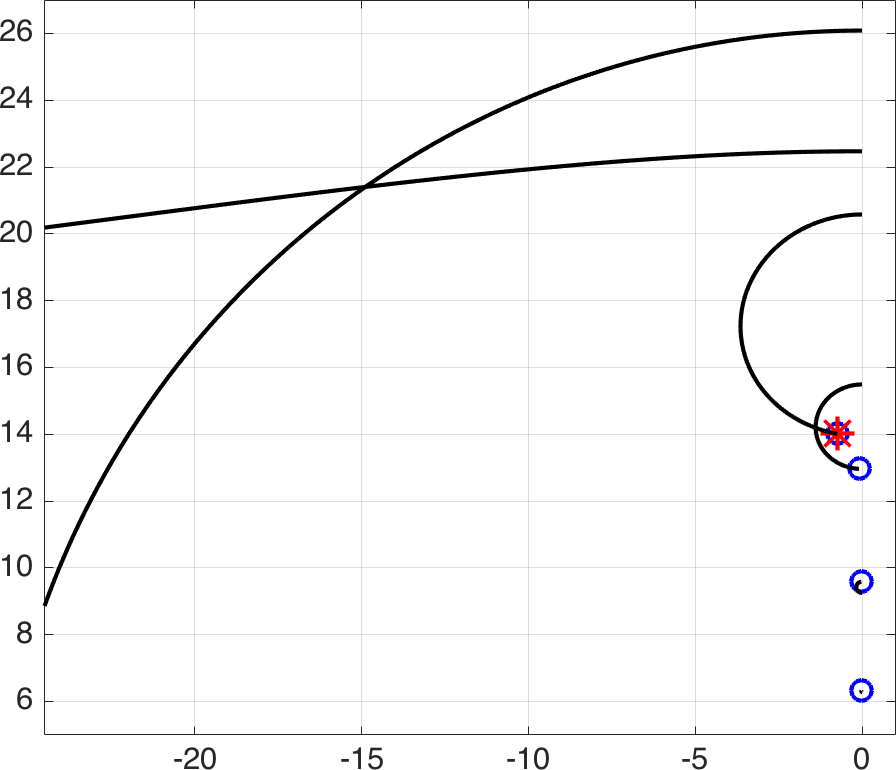
\includegraphics[width=.32\textwidth]{figs/tauEigs3.png}}\\
\subfloat[$\tau = 0$]{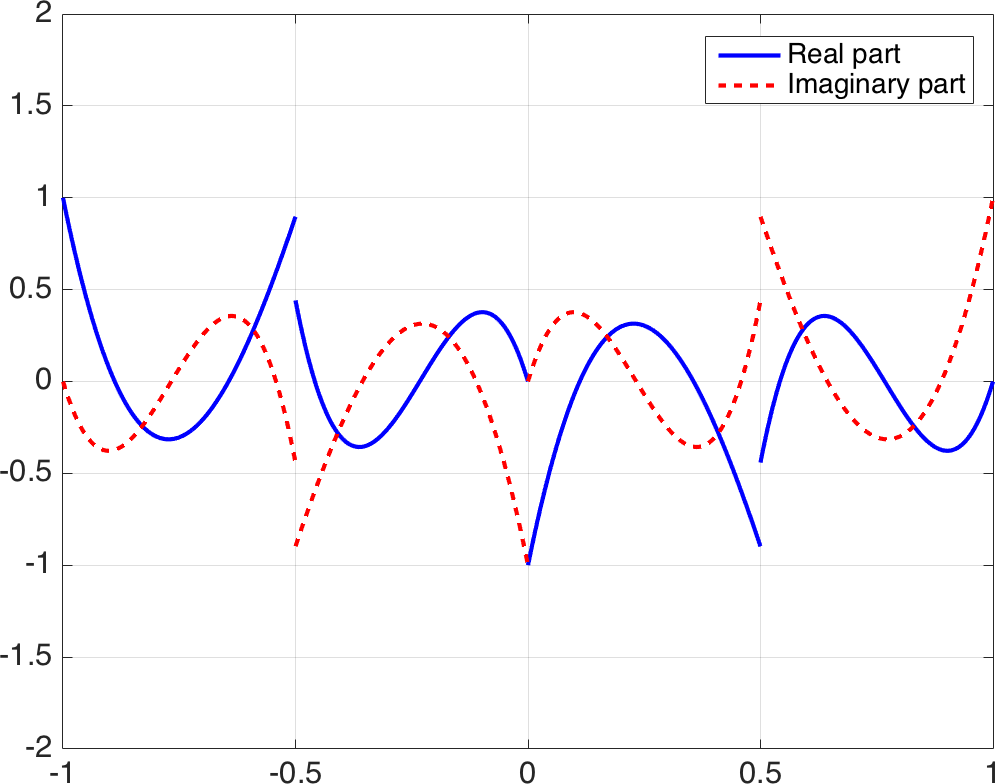
\includegraphics[width=.32\textwidth]{figs/tauModes1.png}}
\hspace{.5em}
\subfloat[$\tau = 1$]{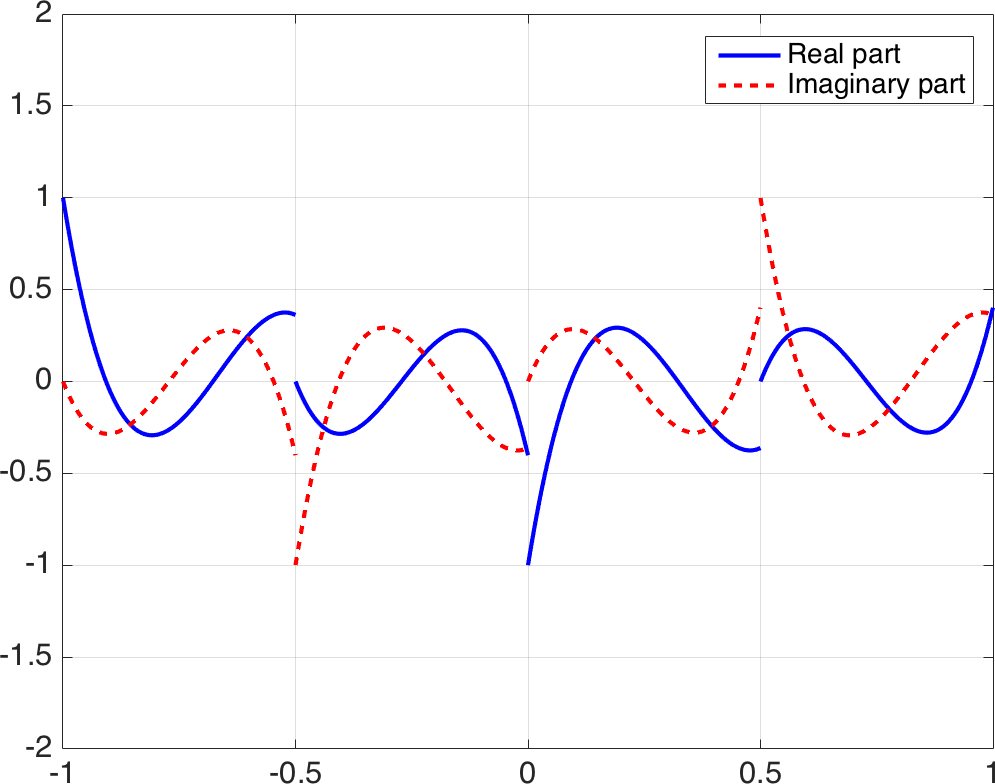
\includegraphics[width=.32\textwidth]{figs/tauModes2.png}}
\hspace{.5em}
\subfloat[$\tau = 10$]{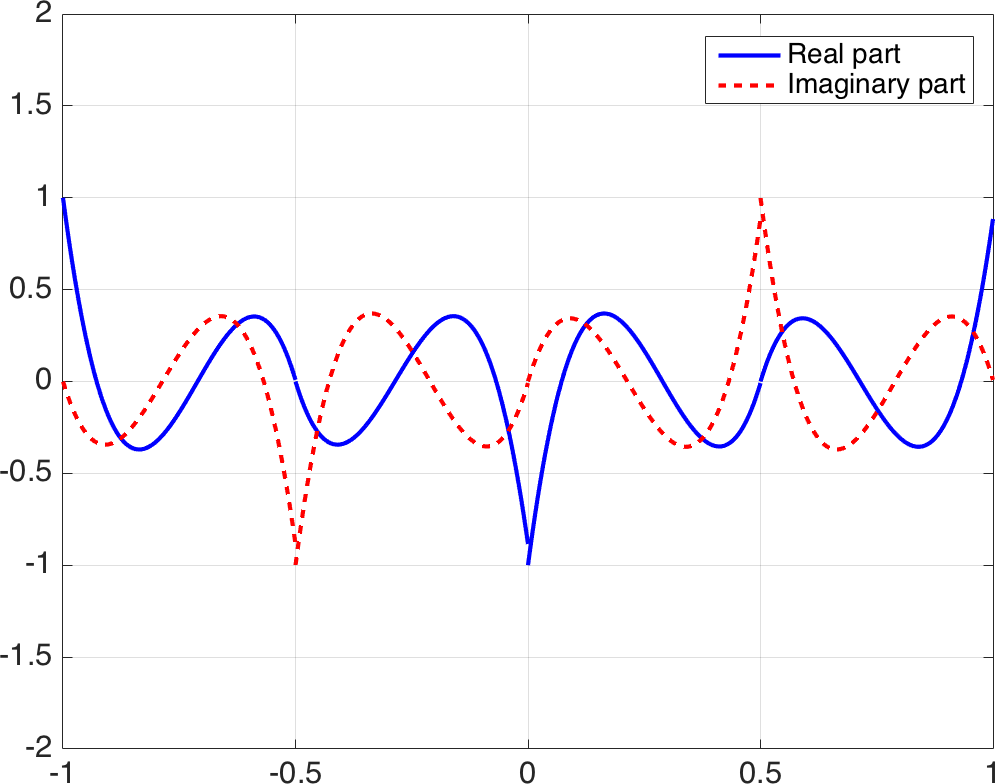
\includegraphics[width=.32\textwidth]{figs/tauModes3.png}}
\caption{Return behavior of DG advection eigenvalues for sufficiently large $\tau$.  For $\tau = 1$ certain eigenvalues have negative real part, and the corresponding eigenmodes are damped.  For $\tau \gg 1$, certain eigenvalues return to the imaginary axis as spurious modes in conforming discretizations. }
\label{fig:spurious}
\end{figure}

We repeat the above experiment for the acoustic wave equation in 1D with reflection boundary conditions on $[-1,1]$, and compare against the exact eigenvalues $\lambda_i = i \frac{\pi}{2}$ for $i = 1,2,\ldots$.  The behavior of the eigenvalues as $\tau$ increases (Figure~\ref{fig:trackModesWave}) is similar to the behavior observed for the scalar advection equation.  An examination of the eigenmodes corresponding to divergent and spurious eigenvalues as $\tau \rightarrow \infty$ shows that these modes behave similarly to the spurious modes observed for the scalar advection equation, with individual pressure and velocity components converging to continuous functions.    

%\begin{figure}
%\centering
%\subfloat{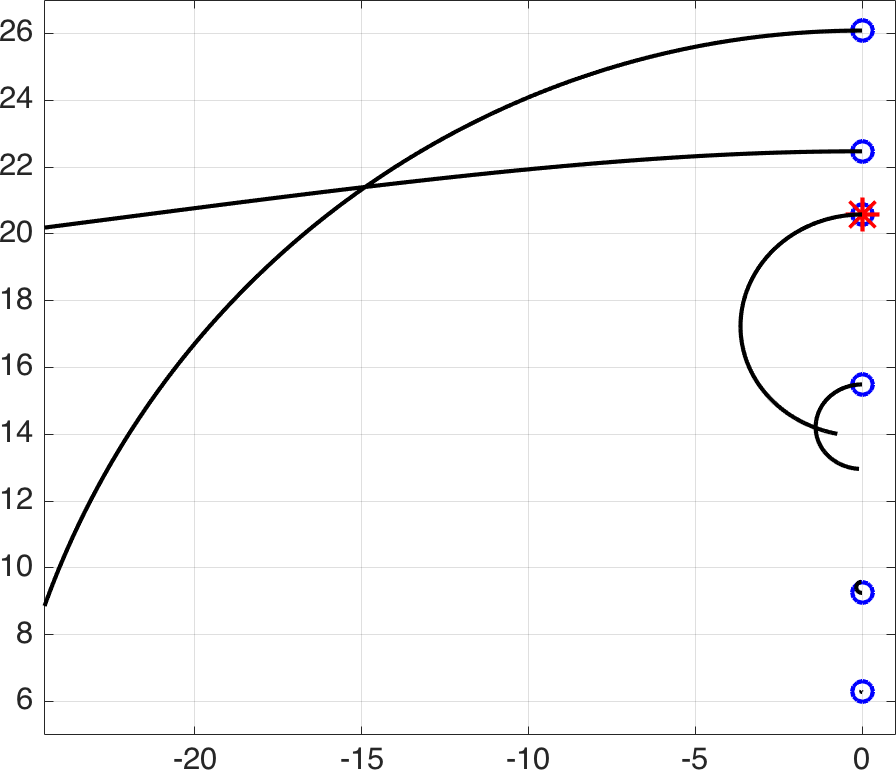
\includegraphics[width=.475\textwidth]{figs/tauEigs1.png}}
%\hspace{.5em}
%\subfloat{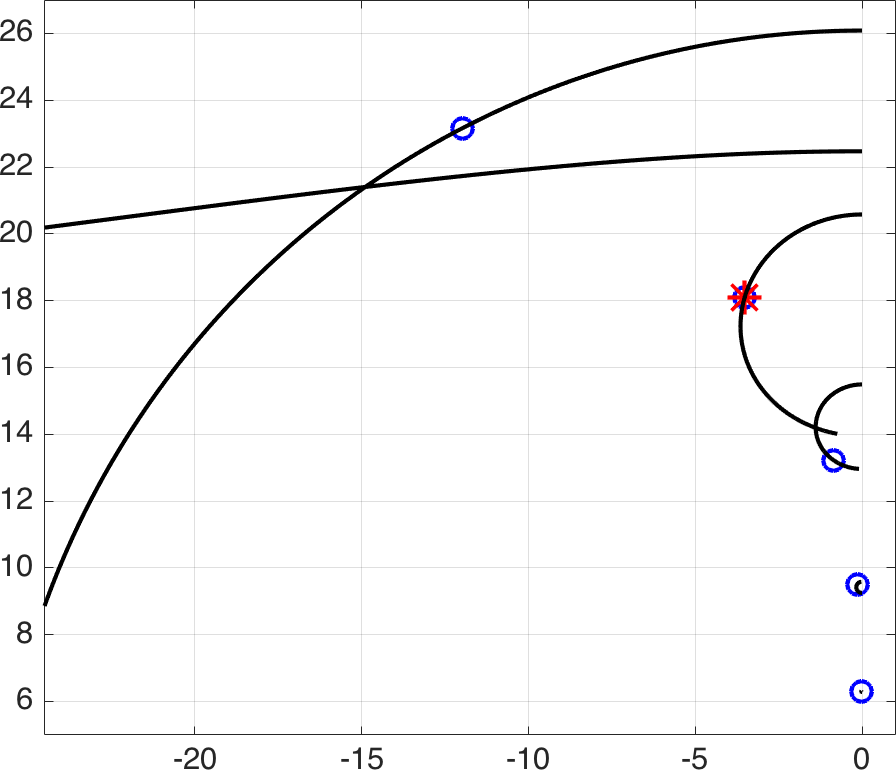
\includegraphics[width=.475\textwidth]{figs/tauEigs2.png}}
%\caption{ }
%\label{fig:trackModesWave}
%\end{figure}

\subsection{2D experiments}

In two space dimensions, taking $\tau\rightarrow \infty$ again results in spurious modes which return to the imaginary axis, with the corresponding eigenmodes approaching conforming functions.  
We illustrate this through numerical experiments for the acoustic wave equation and advection in two space dimensions.  In all numerical experiments, we use $N=3$ and a uniform triangular mesh resulting from bisecting each element of a $2\times 2$ uniform quadrilateral mesh.  

Figure~\ref{fig:waveeigs} shows the spectra of the DG discretization matrix for the acoustic wave equation for $\tau = 1, 10, 50$.  Like the one-dimensional case, a subset of eigenvalues diverge towards the left half plane as $\tau$ increases.  However, unlike the one-dimensional case, these eigenvalues collapse towards the real line as $\tau$ increases.  


\begin{figure}
\centering
\subfloat[$\tau = 1$]{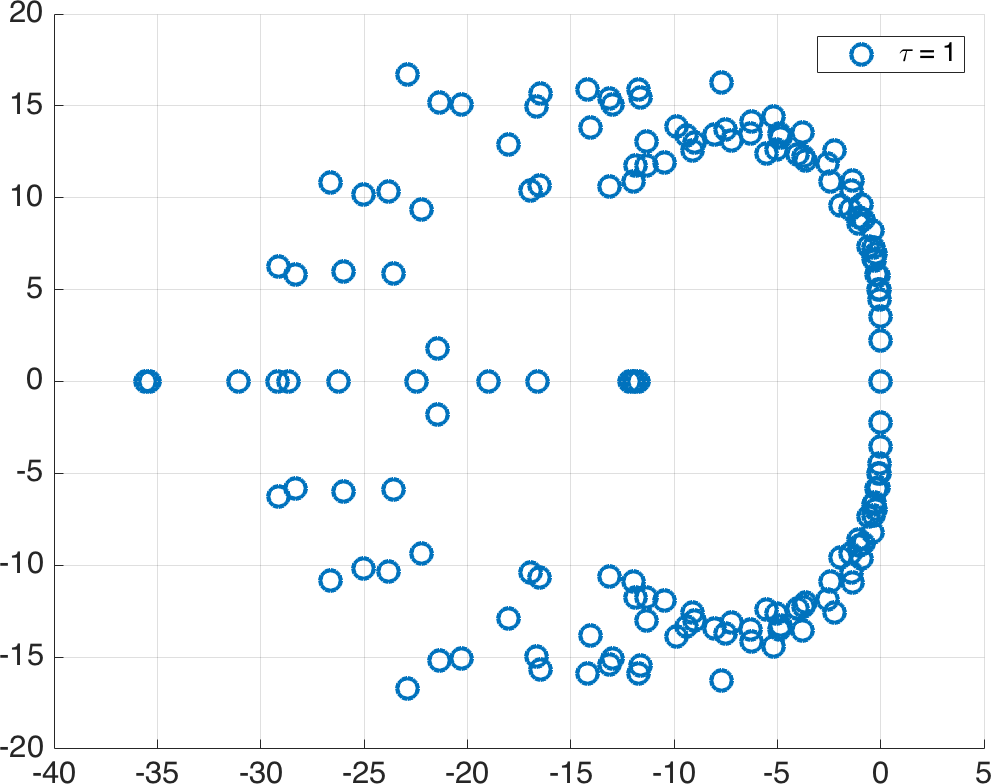
\includegraphics[width=.3\textwidth]{figs/waveEigs1.png}}
\hspace{.5em}
\subfloat[$\tau = 10$]{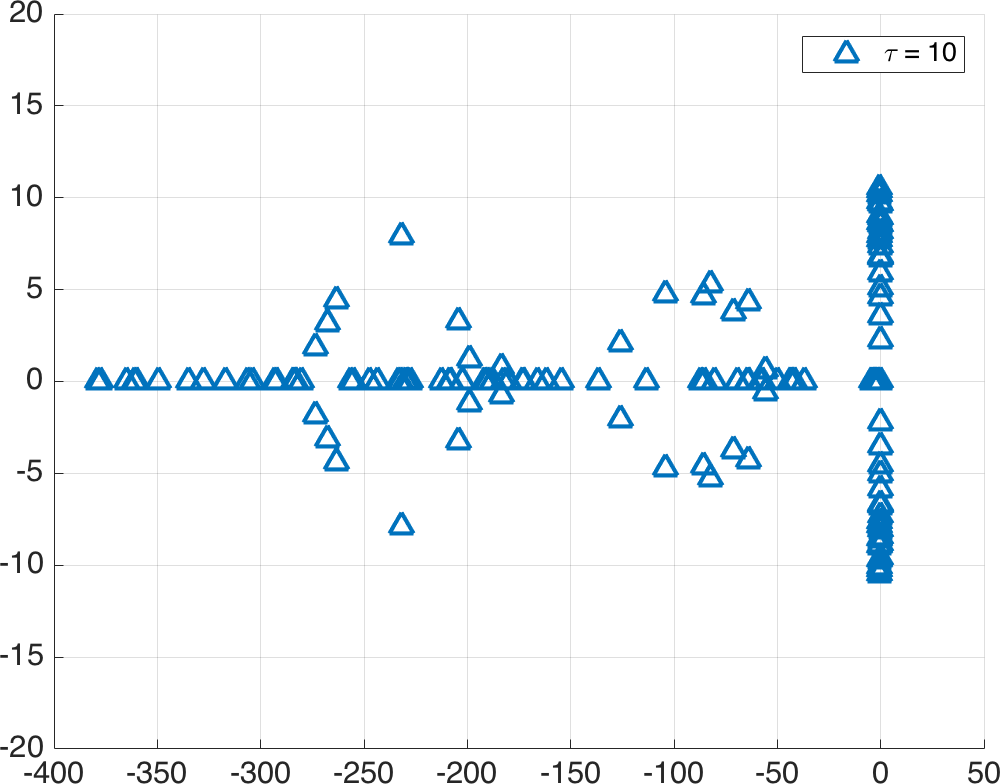
\includegraphics[width=.3\textwidth]{figs/waveEigs2.png}}
\hspace{.5em}
\subfloat[$\tau = 100$]{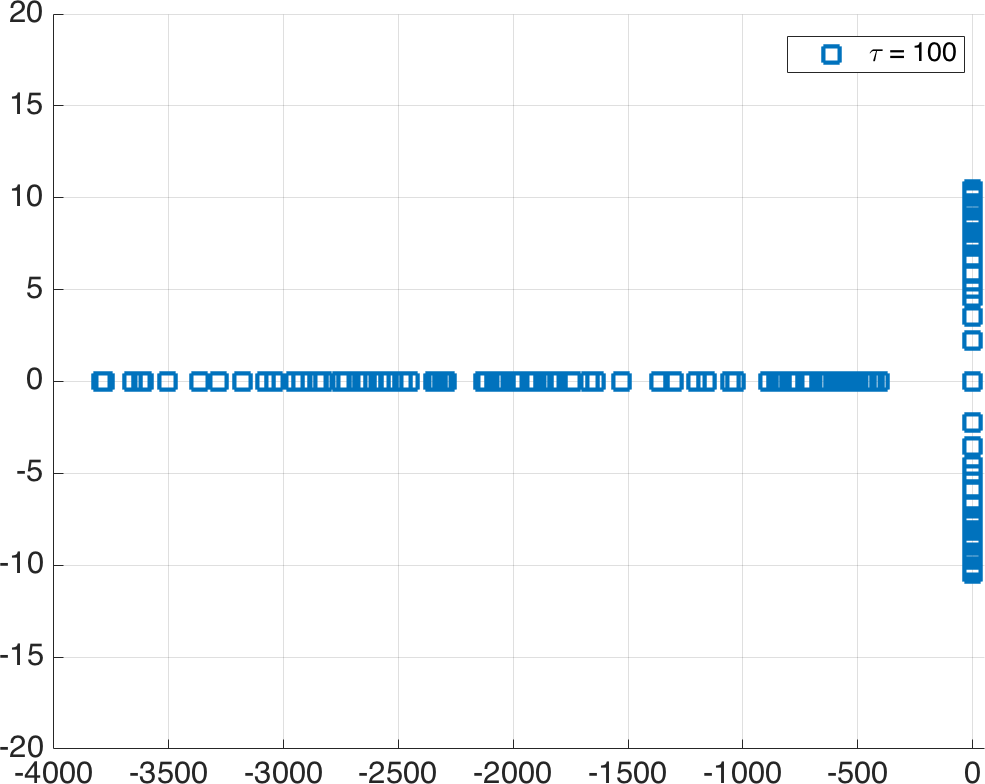
\includegraphics[width=.3\textwidth]{figs/waveEigs3.png}}
\caption{Behavior of eigenvalues for the acoustic wave equation in two dimensions. Note the changing scale of the real axis.}
\label{fig:waveeigs}
\end{figure}

Similarly, as predicted, a subset of eigenvalues returns towards the imaginary axis as $\tau \rightarrow \infty$.  These are shown in Figure~\ref{fig:trackEigsWave}, along with traced paths taken by each eigenvalue as $\tau$ increases.  

\begin{figure}
\centering
\subfloat[$\tau = 0,1, 50$, zoomed in view]{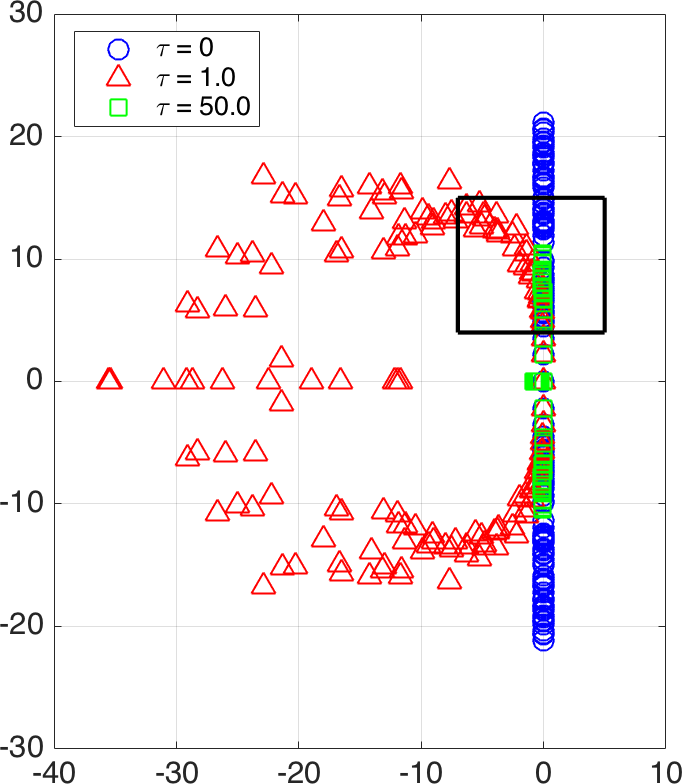
\includegraphics[height=.3\textheight]{figs/waveEigs2Dbox.png}\label{subfig:big}}
\hspace{2em}
\subfloat[$\tau= 0,1,50$, returning eigenvalue paths]{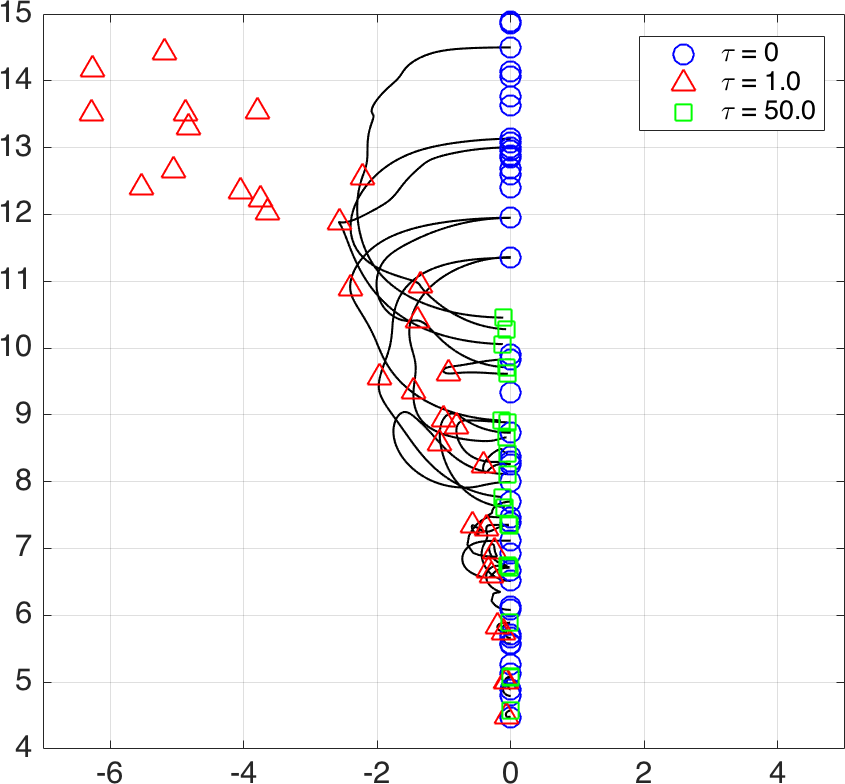
\includegraphics[height=.3\textheight]{figs/trackedWaveEigs2D.png}\label{subfig:box}}
\caption{Behavior of eigenvalues for the acoustic wave equation in two dimensions.  Figure~\ref{subfig:box} shows a zoom of the boxed region in Figure~\ref{subfig:big}, with overlaid eigenvalue paths as $\tau$ increases.  Divergent eigenvalues in the far left half plane are not shown.  }
\label{fig:trackEigsWave}
\end{figure}

The pressure and velocity components of the corresponding acoustic eigenmodes converge to conforming approximations.  As noted in Section~\ref{sec:confexamples}, this implies that pressure components lie in $H^1(\Oh)$ and are continuous across faces, edges, and vertices.  Figure~\ref{fig:trackModesWave} shows the behavior of the pressure component of an eigenmode corresponding to a spurious returning eigenvalue for $\tau = .1, 1, 100$.  As $\tau$ increases and the eigenvalue approaches the imaginary axis, the eigenmode approaches a $C^0$ continuous function with a high frequencies and sharp peak, similar to the spurious eigenmodes observed for the one-dimensional case in Figure~\ref{fig:spurious}.

\begin{figure}
\centering
\subfloat[$\tau = .1$, $\lambda = -0.2379 + 8.7528i$]{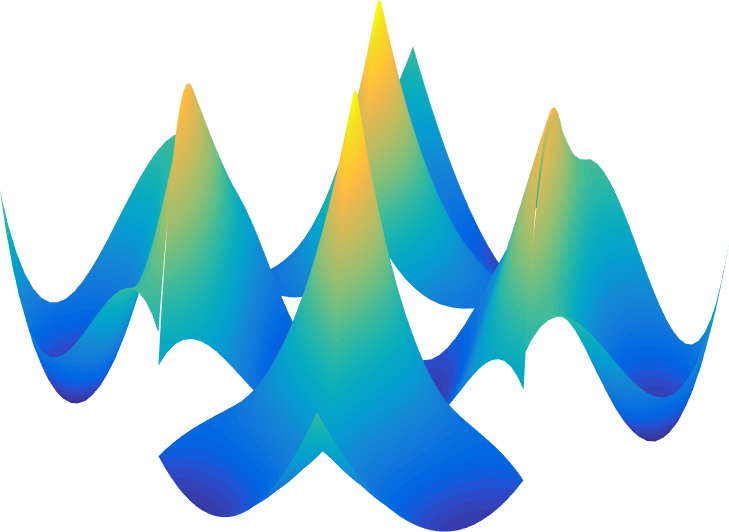
\includegraphics[width=.3\textwidth]{figs/waveEig2D_p1.png}}
\hspace{.5em}
\subfloat[$\tau = 1$, $\lambda = -1.0145 + 8.9270i$]{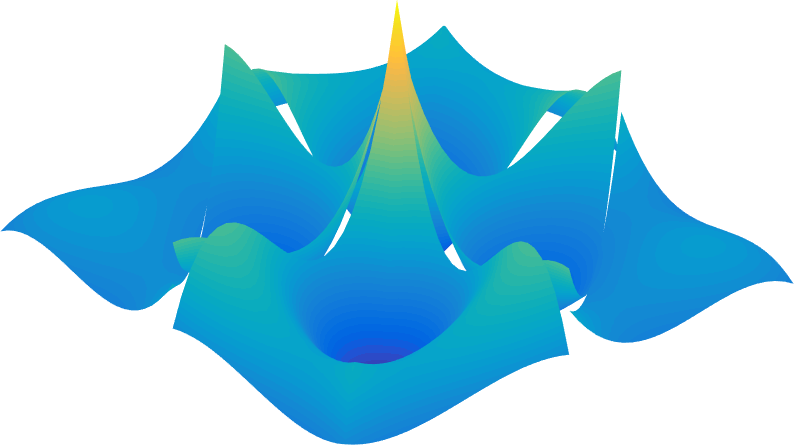
\includegraphics[width=.3\textwidth]{figs/waveEig2D_p2.png}}
\hspace{.5em}
\subfloat[$\tau = 100$, $\lambda = -0.0437 + 7.6167i$]{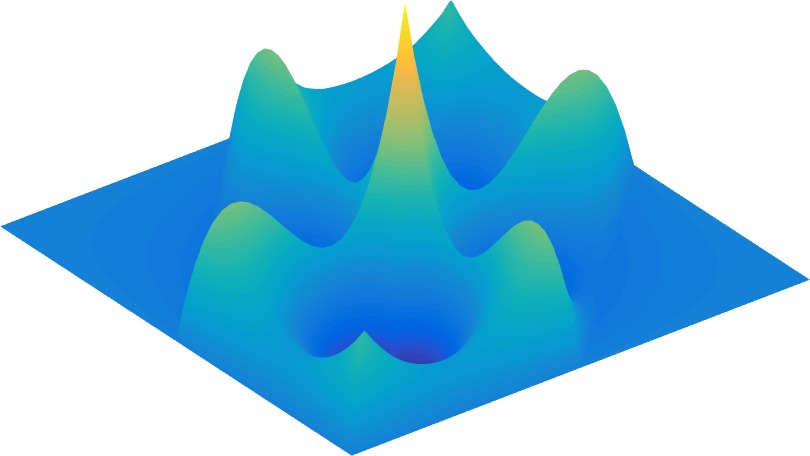
\includegraphics[width=.3\textwidth]{figs/waveEig2D_p3.png}}
\caption{Behavior of the real part of the pressure component of spurious eigenmodes for the acoustic wave equation in two dimensions.  }
\label{fig:trackModesWave}
\end{figure}

The non-zero velocity components of spurious eigenmodes converge to approximations in $H({\rm div}; \Oh)$, such that only the normal component of velocity is continuous across faces.  Figure~\ref{fig:trackModesWaveU} shows visualizations of these eigenmodes.  For large $\tau$, normal jumps of the velocity component vanish.  % approach an $H({\rm div};\Oh)$-conforming approximation.  

\begin{figure}
\centering
\subfloat[$\tau = .1$, $\lambda = -0.6009 +11.3209i$]{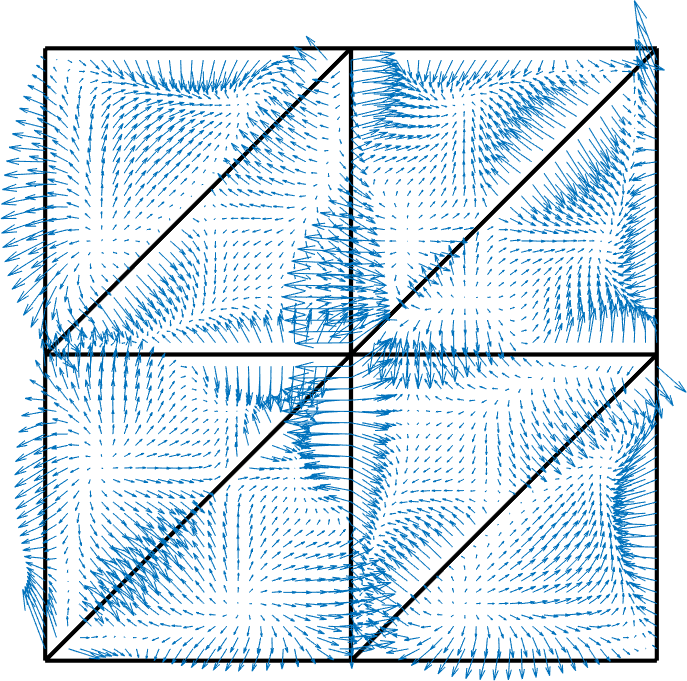
\includegraphics[width=.3\textwidth]{figs/waveEig2D_u1.png}}
\hspace{.5em}
\subfloat[$\tau = 1$, $\lambda =  -1.9601 + 9.5629i$]{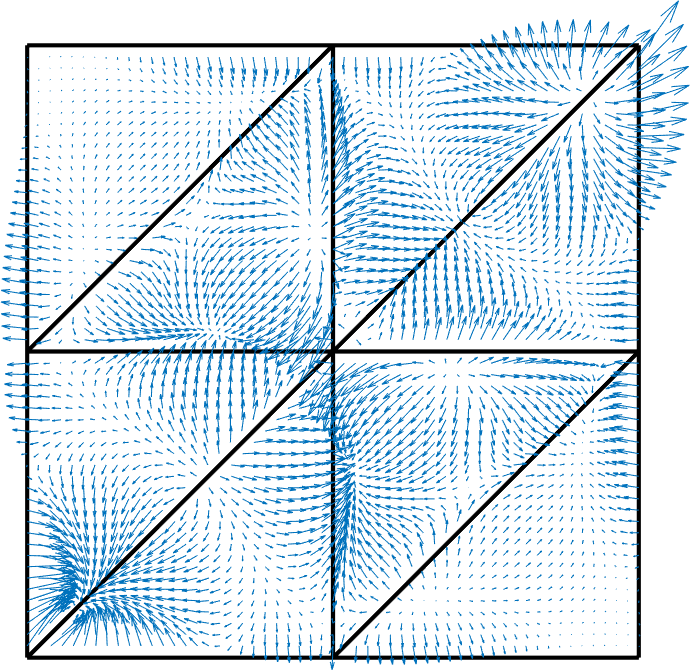
\includegraphics[width=.3\textwidth]{figs/waveEig2D_u2.png}}
\hspace{.5em}
\subfloat[$\tau = 100$, $\lambda = -0.0634 + 7.7670i$]{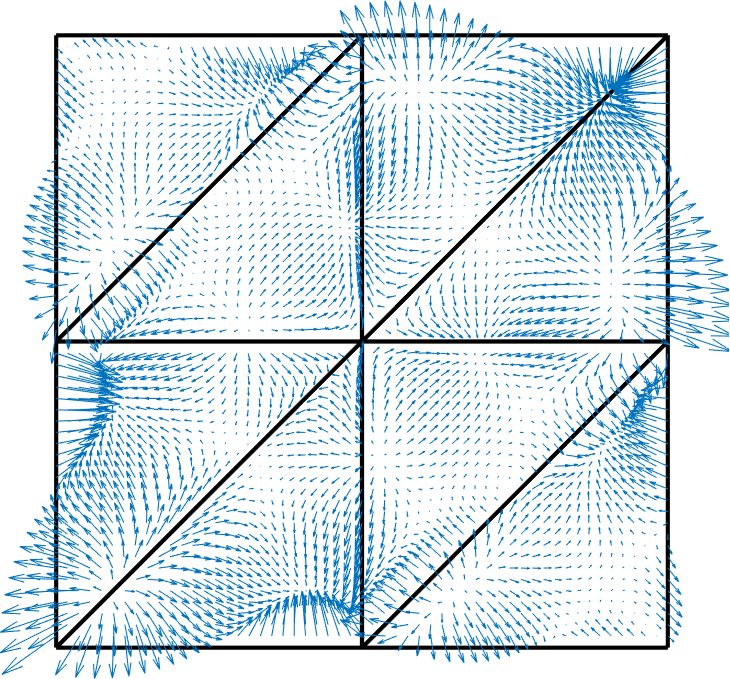
\includegraphics[width=.3\textwidth]{figs/waveEig2D_u3.png}}
\caption{Behavior of the real part of the velocity component of spurious eigenmodes for the acoustic wave equation in two dimensions.  }
\label{fig:trackModesWaveU}
\end{figure}


For the advection equation with periodic boundary conditions, the spectra of the DG discretization behaves similarly.  In all following experiments, we use advection vector $\beta = (1,0)$.  For $\tau=0$, all eigenvalues lie on the imaginary axis, and as $\tau$ increases, the spectra splits into eigenvalues which diverge towards the left half plane and eigenvalues which return to the imaginary axis.  Figure~\ref{fig:trackModesAdvec} shows the spectra of the DG matrix for $\tau = 0,1,50$, with eigenvalue paths for increasing values of $\tau$ overlaid.  

\begin{figure}
\centering
\subfloat{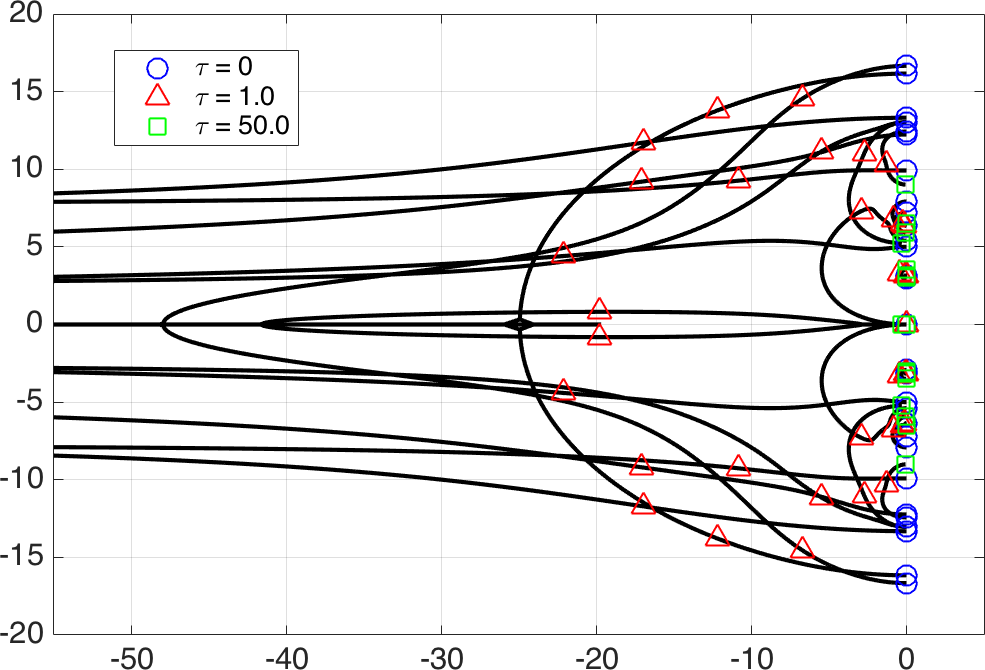
\includegraphics[width=.475\textwidth]{figs/trackedAdvecEigs.png}}
\hspace{.5em}
\subfloat{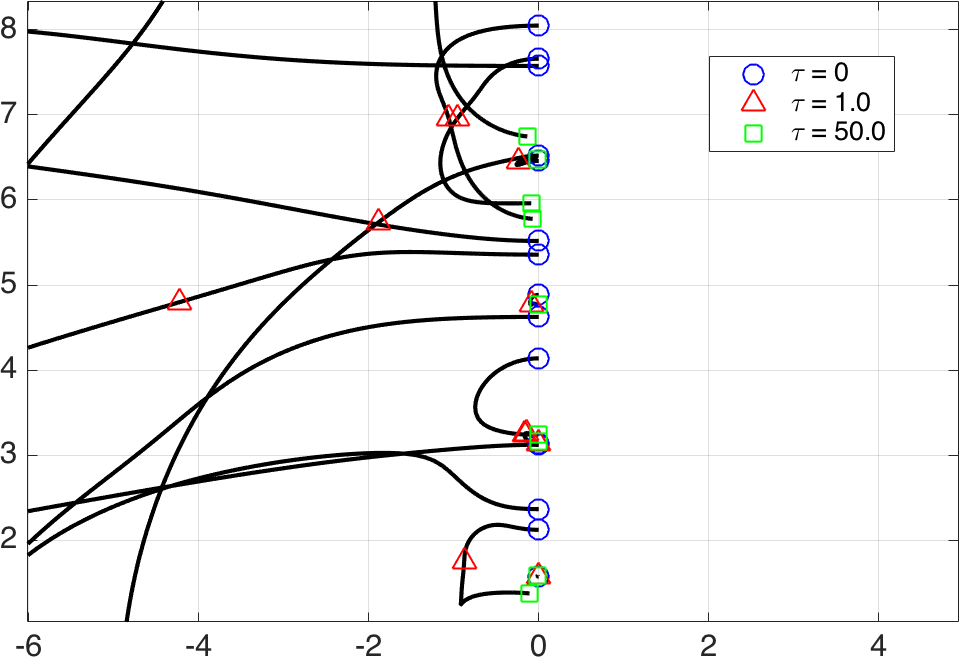
\includegraphics[width=.465\textwidth]{figs/trackedAdvecEigsZoom1.png}}
\caption{Eigenvalue paths for the DG discretization of advection as $\tau$ increases.  Divergent eigenvalues in the far left half plane are not shown.  }
\label{fig:trackModesAdvec}
\end{figure}

Unlike spurious conforming modes present for the acoustic wave equation, spurious conforming modes for the advection equation satisfy $\jump{\beta_n u} = 0$, and allow discontinuities along faces which are tangential to flow directions.  \note{Find cite on regularity of advection solutions.} 

\begin{figure}
\centering
\subfloat[$\tau = 0$, $\lambda = 0 + 7.9246i$]{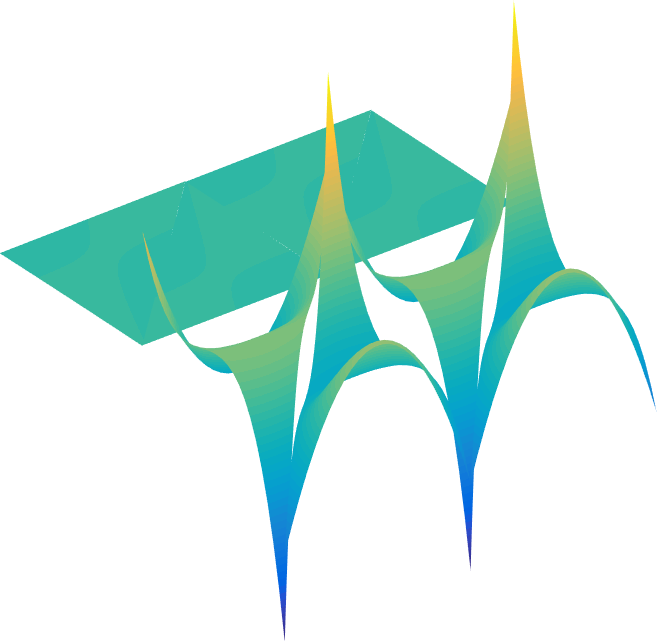
\includegraphics[width=.3\textwidth]{figs/advecEig2D_u1.png}}
\hspace{.5em}
\subfloat[$\tau = 1$, $\lambda =  -0.8278 + 6.7831i$]{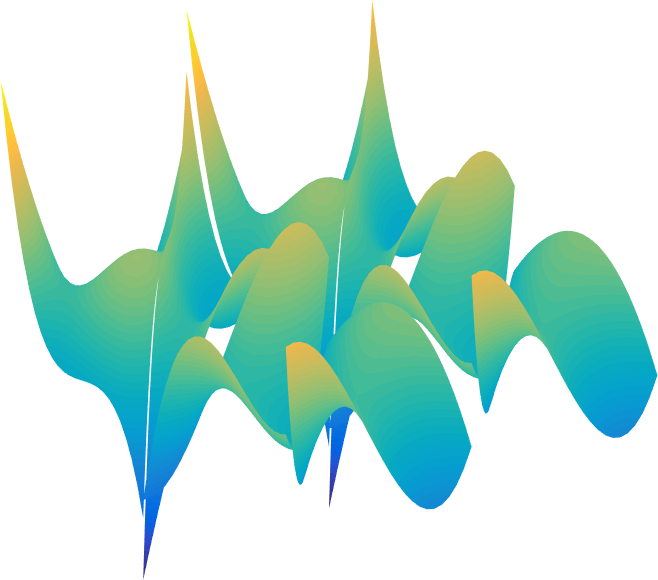
\includegraphics[width=.3\textwidth]{figs/advecEig2D_u2.png}}
\hspace{.5em}
\subfloat[$\tau = 100$, $\lambda = -0.0239 + 5.9282i$]{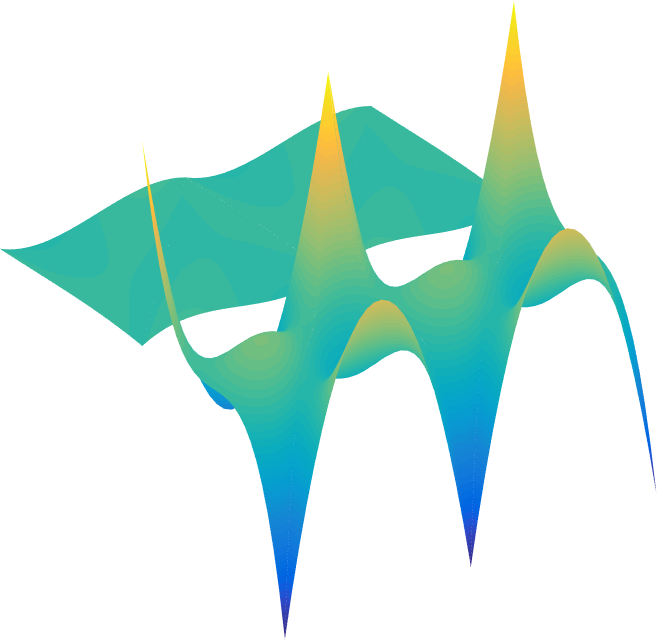
\includegraphics[width=.3\textwidth]{figs/advecEig2D_u3.png}}
\caption{Behavior of the real part of spurious eigenmodes for the advection equation with $\beta = (1,0)$. }
\label{fig:trackModesAdvecU}
\end{figure}

\section{Conclusions}

\note{Penalized DG methods as sweet spot treatments of spurious modes, somewhere between central DG and conforming discretizations.}

\bibliographystyle{unsrt}
\bibliography{dgpenalty}


\end{document}


